%========ANÁLISIS DEL MODULO DE COMUNICACIÓN=======

\subsection{Módulo de comunicación GSM}
%El módulo de comunicación GSM permitirá el envío de mensajes SMS con la información proporcionada por el microcontrolador. \\
%
%Para determinar el módulo a utilizar, se consideraron únicamente módulos con el chip integrado ya que proporciona la ventaja de contener todos los elementos que éste requiere. Además al requerir únicamente del envío de SMS se descartaron varios modelos encontrados. \\
%
%Finalmente se realizó una tabla comparativa entre los módulos con el nombre GSMx Click de la empresa MikroElektronika que corresponden a los requerimientos buscados. \\
%
%Las principales características a considerar para la selección del módulo fueron la banda soportada y las interfaces de comunicación que ofrece. Adicionalmente se consideraron el voltaje y precio. \\
%
%En la Tabla \ref{analisis:moduloGSM} se muestran los datos de los diferentes módulos de comunicación GSM para cada característica.\\
%
%\begin{table}[htbp]
%	\begin{center}
%		\scalebox{0.93}[0.95]{
%		\begin{tabular}{|c|c|c|c|c|c|}
%			\hline
%			%			\rowcolor{colorSecundario}
%			%			\color{green}
%			\thead{Modelo}&\thead{Fabricante}&\thead{Frecuencia de banda\\(MHz)}&\thead{Interfaces}&\thead{Voltaje \\ (V)}&\thead{Precio\\(USD)}\\
%			\hline
%			\hline
%			GL865-QUAD & Telit&850/900/1800/1900&UART&3.22 - 4.5&49.0\\
%			\hline
%			M95 & Quectel&850/900/1800/1900&GPIO/UART&3.3 - 4.6& 44.0\\
%			\hline
%			SIM800H & SIMcom&850/900/1800/1900&GPIO/UART&3.4 - 4.4&57.0\\
%			\hline
%			SARA-G3 & ublox&900/1800&GPIO/UART/USB&4&74.0\\
%			\hline
%		\end{tabular}}
%		\caption{Comparativa de módulos GSM.}
%		\label{analisis:moduloGSM}
%	\end{center}
%\end{table}
%	
%Debido a que para realizar pruebas se utilizará una tarjeta SIM de algún operador celular del país se consideraron las operadoras más utilizadas a nivel nacional con las frecuencias de operación de sus bandas. \cite{garrido2018} \\ 
%
%Al no requerir de una gran velocidad para el envío de datos se consideró usar la red 3G.\\
%
%En la Tabla \ref{analisis:moduloGSMFrecuencias} se muestran los datos de las diferentes operadoras.\\
%
%\begin{table}[htbp]
%	\begin{center}
%		\scalebox{0.93}[0.95]{
%			\begin{tabular}{|c|c|}
%				\hline
%				\thead{Operador}&\thead{Frecuencia para 3G (MHz)}\\
%				\hline
%				\hline
%				AT\&T (Iusacell y Nextel) & 850/1700/1900/2100\\
%				\hline
%				Movistar & 850/1900\\
%				\hline
%				Telcel & 850/1900\\
%				\hline
%			\end{tabular}
%		}
%		\caption{Frecuencias de banda de operadoras celulares.}
%		\label{analisis:moduloGSMFrecuencias}
%	\end{center}
%\end{table}
%
%Por las características que presenta y el soporte que tiene en la red 3G nacional, se decidió utilizar el módulo \textbf{GSM Click} con el chip \textbf{GL865-QUAD} de Télit, mostrado en la figura \ref{fig:AnalisisGSM}.\\
%
%		\begin{figure}[htbp!]
%			\centering
%			\fbox{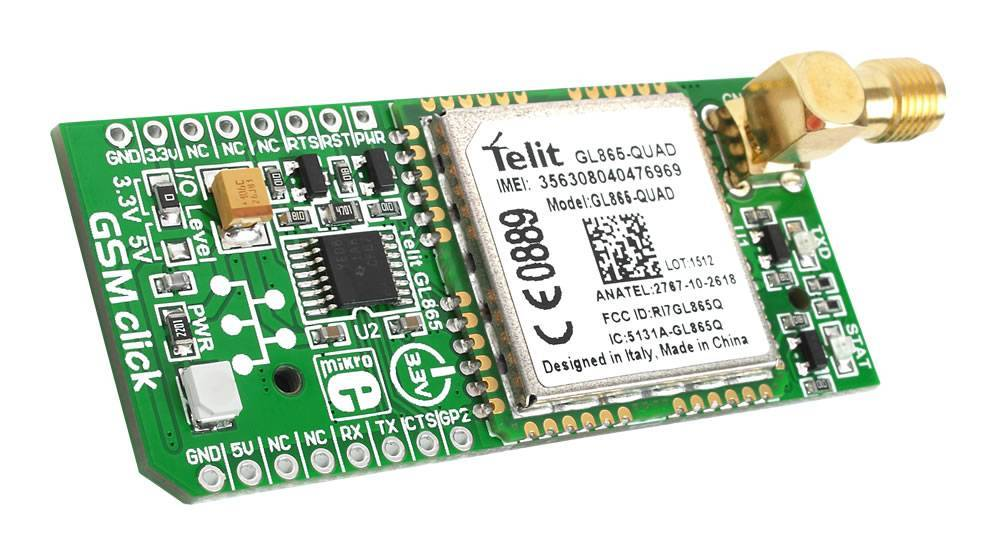
\includegraphics[width=0.6\textwidth]{Analisis/imagenes/gsm.jpg}}
%			\caption{GSM Click}
%			\label{fig:AnalisisGSM}
%		\end{figure}
%		
%		\clearpage